\chapter{Scomposizione del VAB}
\section{Considerazioni iniziali}
Per il calcolo delle equazioni dinamiche del sistema siamo andati a considerare ogni singolo corpo rigido componente il sistema, calcolandone le grandezze fisiche di posizione e velocità, seguendo un approccio cartesiano. 
Nello specifico abbiamo considerato il sistema composto da:
\begin{itemize}
	\item Asta
	\item Utente a bordo dello chassis
	\item Chassis (nel corso della trattazione sarà chiamata talvolta anche base)
	\item Ruota (che poi sarà considerata con un contributo, essendo il VAB composto da due ruote)
\end{itemize}

Ognuno di questi corpi rigidi separati è individuato da un punto, che ne rappresenta il centro di massa (o baricentro del corpo stesso): avremo quindi questo insieme di punti caratterizzanti il sistema (figura ~\ref{fig:VAB_baricentri})

\begin{itemize}
	\item \textbf{$P_a$}
	\item \textbf{$P_b$}
	\item \textbf{$P_c$}
	\item \textbf{$P_r$}
\end{itemize}

\begin{figure}[h]
	\centering   	
	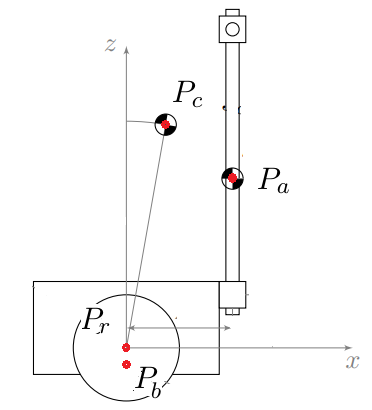
\includegraphics[width=0.4\textwidth]{Immagini/VAB_baricentrum.png}
	\caption{Baricentri dei singoli corpi rigidi}
	\label{fig:VAB_baricentri}
\end{figure} 

\section{Grandezze di supporto}
Prima di andare a definire le componenti di energia potenziale e cinetica di ogni singolo corpo, siamo andati ad introdurre alcune grandezze geometriche di supporto che definiremo qui di seguito.

Nello specifico abbiamo introdotto i seguenti parametri, specificati anche in figura ~\ref{fig:VAB_lunghezze}:
\begin{itemize}
	\item \textbf{$l_a$}: rappresenta la congiungente tra il centro del sistema di riferimento e il centro dell'asta, utilizzata appunto come manubrio, che abbiamo individuato come
	\begin{center}
		{\Large $\sqrt{(\frac{h_a}{2} + \frac{h_b}{2})^2 + (\frac{w_b}{2})^2}$}
	\end{center}
	\item \textbf{$l_c$}: (TODO: check) questa grandezza invece rappresenta per noi l'altezza del baricentro del corpo dell'utente, la quale ovviamente andrà a dipendere dal valore di inclinazione del corpo stesso.
	Considerando il corpo inzialmente in posizione verticale, avremo che questa grandezza corrisponde alla congiungente dal centro del sistema di riferimento al punto $P_c$, che equivale a dire che
	\begin{center}
		$l_c = 0.55\bullet h_c + \frac{h_b}{2}$
	\end{center}
	\item \textbf{$l_b$}: spostamento verso il basso, lungo l'asse z, del baricentro dello chassis. Da specifiche del progetto sappiamo che questa grandezza ha valore (con segno negativo) di:
	\begin{center}
		$l_b = 0.1 m$
	\end{center}
	\item \textbf{$\beta$}: angolo formato con la verticale dalla congiungente tra il centro del sistema di riferimento e il punto $P_a$. Si ricava, con un semplice approccio trigonometrico, che l'angolo in questione ha questa forma
	\begin{center}
		$\arctan{(\frac{\frac{w_b}{2}}{\frac{h_a}{2} + \frac{h_b}{2}})}$
	\end{center}
\end{itemize}

\begin{figure}[h]
	\centering   	
	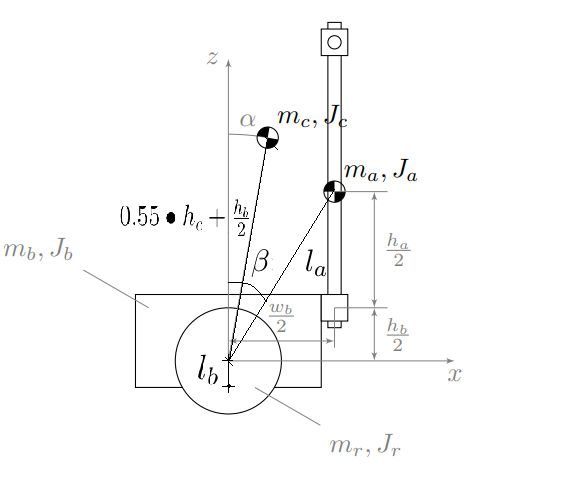
\includegraphics[width=0.4\textwidth]{Immagini/VAB_additionalMeasures.png}
	\caption{Lunghezze di supporto}
	\label{fig:VAB_lunghezze}
\end{figure}

\section{Calcolo componenti dinamiche e potenziali per ogni corpo rigido del sistema}
Per ognuno dei corpi rigidi definiti in precedenza siamo andati appunto a calcolare:

\begin{itemize}
	\item \textbf{Coordinate spaziali P} espresse nel sistema di riferimento XZ. A queste due coordinate cartesiane ne va aggiunta una terza, relativa alle coordinate angolari (per poter tener così conto dei contirbuti inerziali);
	\item \textbf{Vettore delle velocità V} $\rightarrow$ vettore $3\times 1$
	\item \textbf{Matrice delle masse M} $\rightarrow$ matrice $3\times 3$
	\item \textbf{Energia cinetica T} $\rightarrow \frac{1}{2}\bullet V^T \bullet M \bullet V$
	\item \textbf{Energia potenziale U}
	\item \textbf{Lagrangiana \textit{parziale} L}
\end{itemize}

\subsection{Asta}
\begin{itemize}
	\item \textbf{$P_a = \left(\begin{array}{c}
		r\,\phi \left(t\right)+l_a \,\mathrm{sin}\left(\beta +\theta \left(t\right)\right)\\
		l_a \,\mathrm{cos}\left(\beta +\theta \left(t\right)\right)\\
		\theta \left(t\right)
		\end{array}\right)$}

	\item \textbf{$V_a = 	\frac{\partial }{\partial t}\;P_a \left(t\right)
		= \left(\begin{array}{c}
		r\,\dot{\phi}+l_a \,\mathrm{cos}\left(\beta +\theta \left(t\right)\right)\,\dot{\theta}\\\\
		-l_a \,\mathrm{sin}\left(\beta +\theta \left(t\right)\right)\,\dot{\theta}\\\\
		\dot{\theta}
		\end{array}\right)$}
	
	\item Nella stesura della matrice di massa,  \textbf{$M_a = \left(\begin{array}{ccc}
		m_a  & 0 & 0\\
		0 & m_a  & 0\\
		0 & 0 & m_a \,{l_a }^2 +J_a 
		\end{array}\right)$}
	
	\item \textbf{$T_a = m_a \,{l_a }^2 \,{{\left(\frac{\partial }{\partial t}\;\theta \left(t\right)\right)}}^2 +\frac{m_a \,r^2 \,{{\left(\frac{\partial }{\partial t}\;\phi \left(t\right)\right)}}^2 }{2}+\frac{J_a \,{{\left(\frac{\partial }{\partial t}\;\theta \left(t\right)\right)}}^2 }{2}+m_a \,\mathrm{cos}\left(\beta +\theta \left(t\right)\right)\,l_a \,r\,\frac{\partial }{\partial t}\;\theta \left(t\right)\,\frac{\partial }{\partial t}\;\phi \left(t\right)$}
\end{itemize}
\subsection{Chassis}
\subsection{Utente}
\subsection{Ruota}